\Chapter{JavaScript implementáció}

% Kb. 8-12 oldal

\Section{A p5 függvénykönyvtár}

% Fél-egy oldalas áttekintés a p5-ről.

\noindent
Az elkészült szerkesztő jelentős mértékben támaszkodik a p5.js függvénykönyvtár adta lehetőségekre. A p5 oldalán az alábbi ismertető olvasható:


\noindent
\textit{A p5.js egy JavaScript könyvtár a kreatív kódoláshoz, amelynek középpontjában az áll, hogy a kódolást elérhetővé és befogadóvá tegye művészek, tervezők, oktatók, kezdők és bárki más számára! A p5.js ingyenes és nyílt forráskódú, mert hiszünk abban, hogy a szoftvereknek és a tanuláshoz szükséges eszközöknek mindenki számára elérhetőnek kell lenniük.}

\noindent
\textit{A vázlat metaforáját használva a p5.js teljes körű rajzolási funkcionalitással rendelkezik. Azonban nem korlátozódik a rajzvászonra. Az egész böngészőoldalt tekintheted vázlatodnak, beleértve a HTML5-objektumokat a szöveghez, a bevitelhez, a videóhoz, a webkamerához és a hanghoz. }\cite{p5js}

\SubSection{Telepítése}

A p5 függvénykönyvtár telepítéséhez csak hozzá kell adni a fájlunkhoz:

\begin{lstlisting}[style=html]
<html>
	<head>
		<script src="../p5.min.js"></script>
		<script src="sketch.js"></script>
	</head>
	<body>
	</body>
</html>
\end{lstlisting}

\SubSection{Használat}

A p5.js függvényhívások a \textit{sketch.js}-ben kapnak helyet:

\begin{lstlisting}[style=es6]
function setup() {
	
	createCanvas(400, 400);

}
function draw() {
	
	background(220);
	ellipse(50,50,80,80);

}
\end{lstlisting}

\noindent
A \textit{setup} függvény a \textit{sketch.js} betöltésekor fut le, célszerű iderakni a p5 vászon létrehozását (\textit{createCanvas} függvényhívás, mely paraméterként várja a magasságot és a szélességet). A \textit{draw} függvény a futás során folyamatosan meghívódik.


\Section{Az alkalmazás felépítése}

% Blokkdiagram féle, hogy mi hol helyezkedik el az alkalmazásban.

\Section{Definiált osztályok bemutatása}

% UML osztálydiagram.
% Minden osztályról érdemes legalább 1-2 mondatot írni.
% A megvalósítással kapcsolatos tapasztalatokat is lehet itt részletezni.

\begin{figure}[!h]
	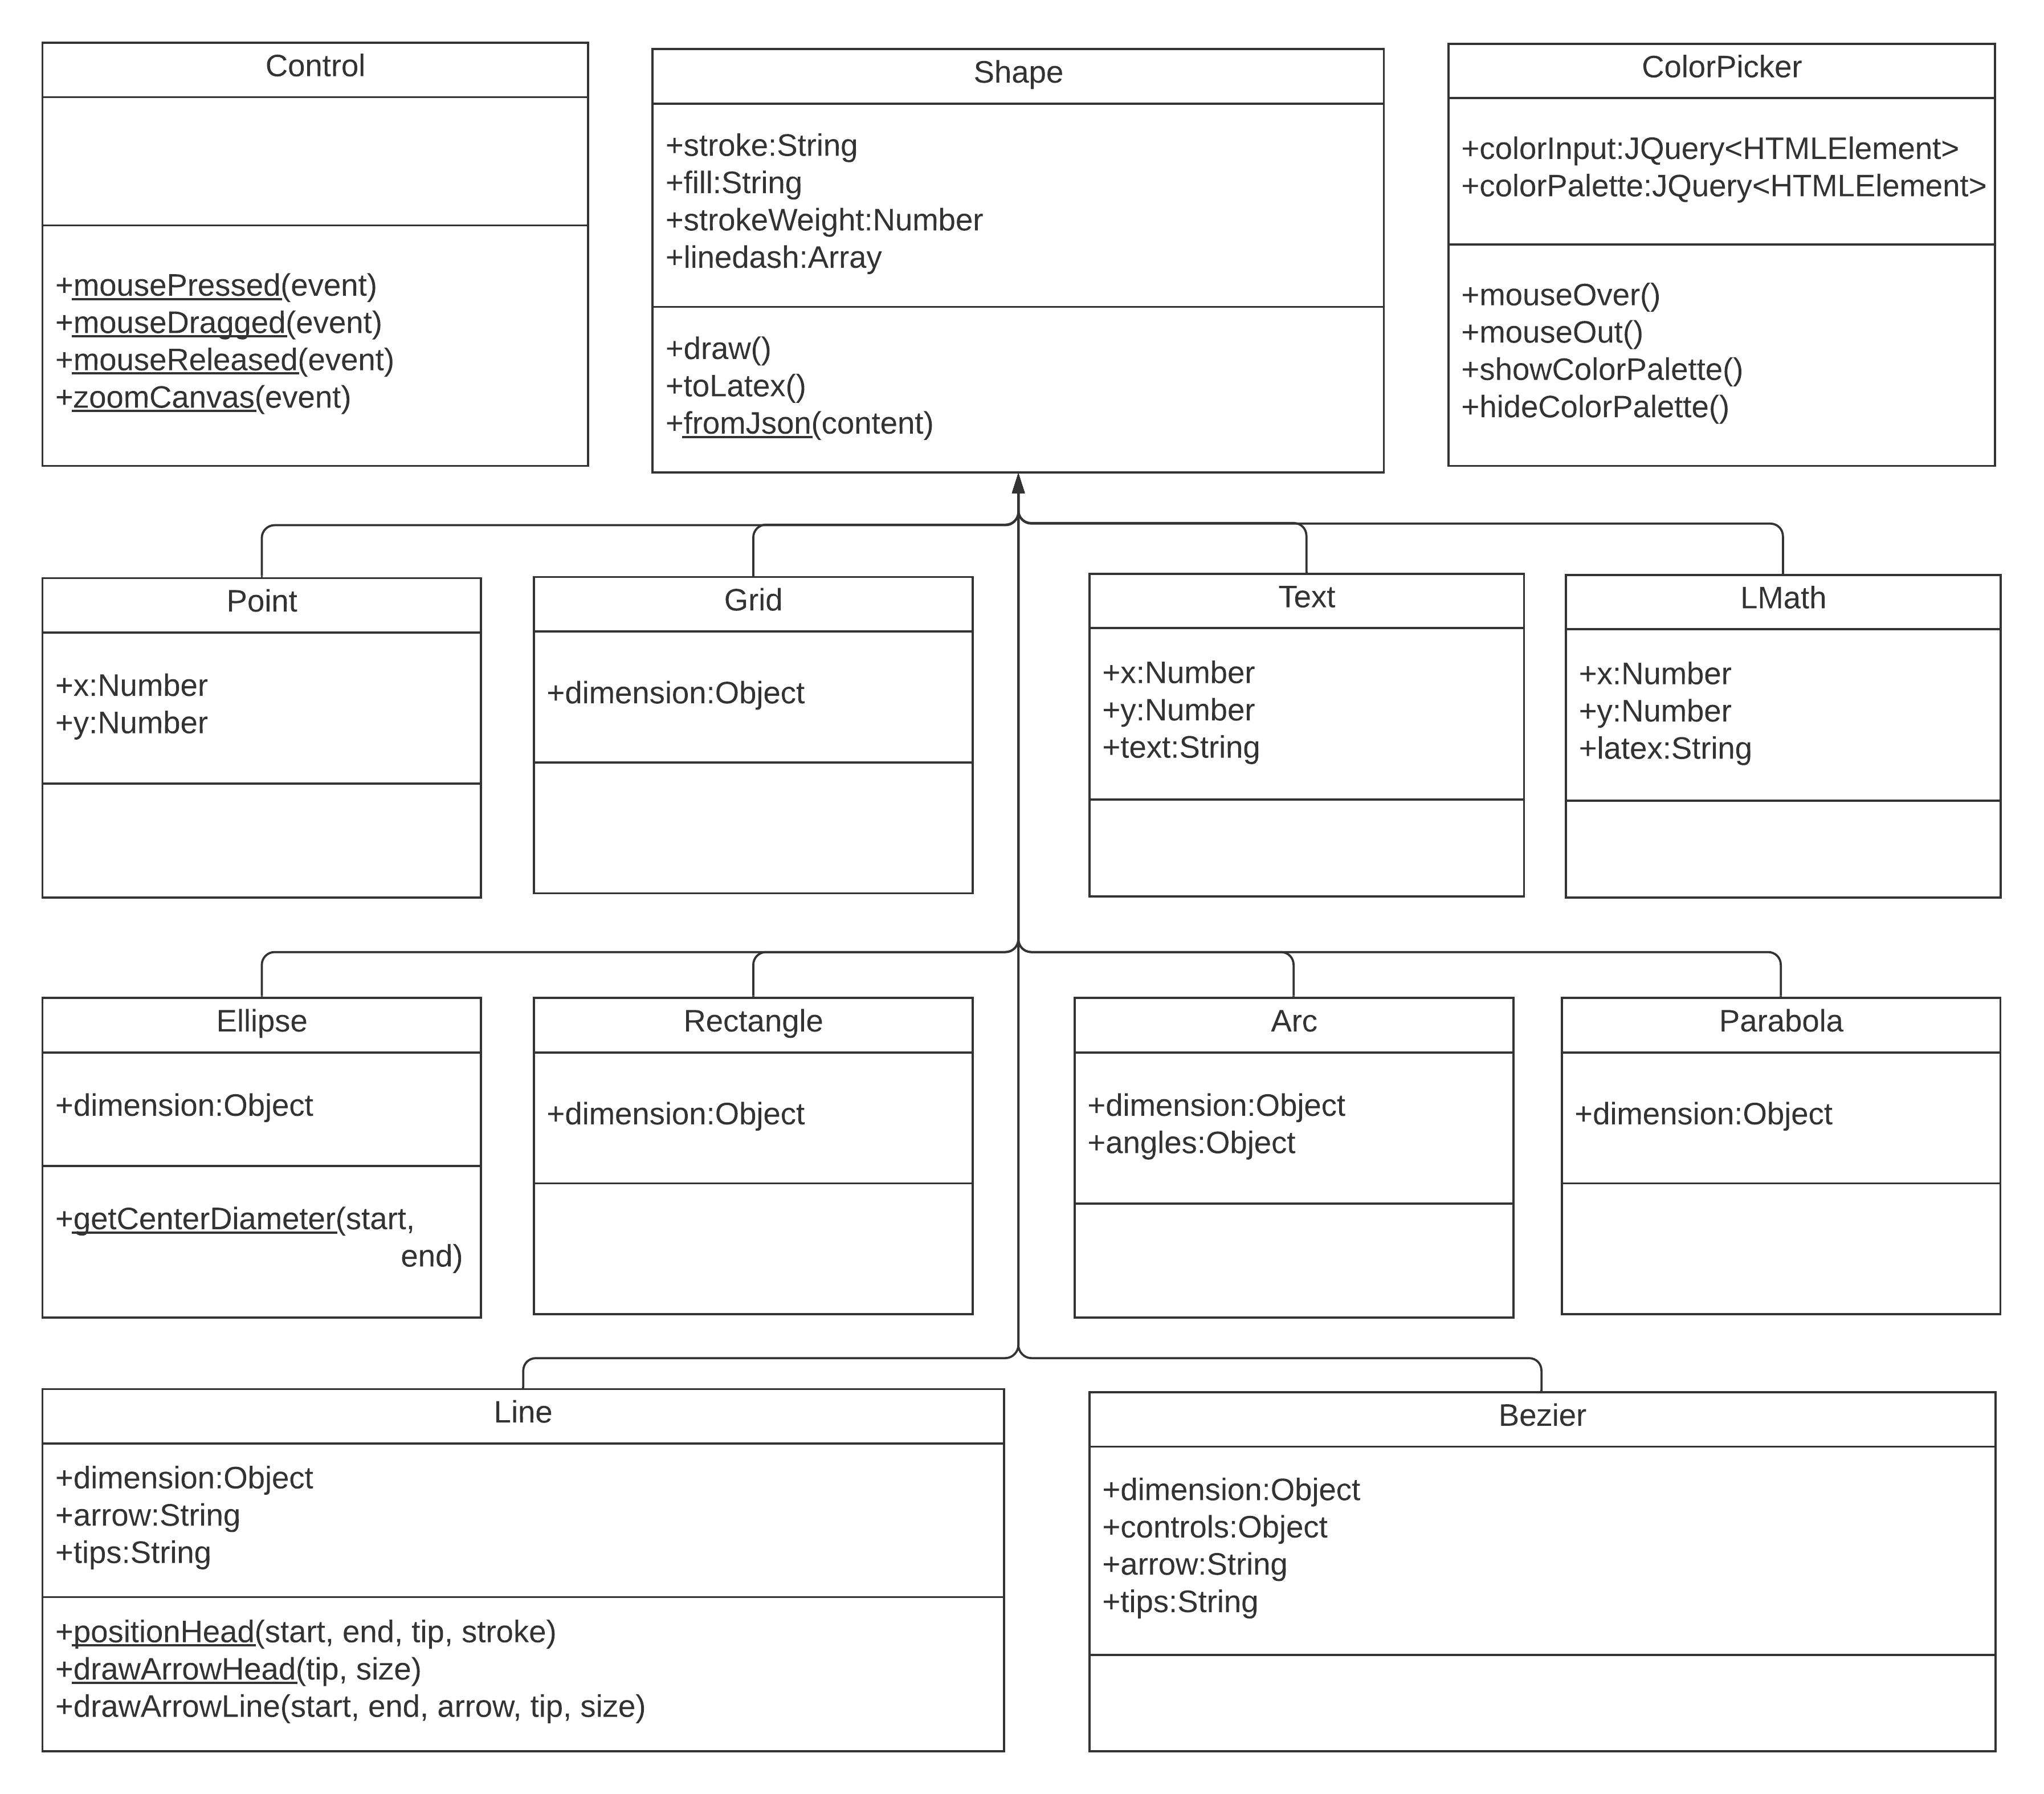
\includegraphics[width=\textwidth]{images/uml.png}
	\caption{Az osztályok UML diagrammja}
	\label{fig:uml1}
\end{figure}


%\begin{lstlisting}[style=ES6]
%\end{lstlisting}